%To compile as handout, use
%pdflatex "\def\ishandout{1} \input{filename.tex}"
%Defaults to non-handout mode (with slide reveals)
\ifdefined\ishandout
  \documentclass[handout]{beamer}
\else
  \documentclass{beamer}
\fi
 
\usetheme[numbering = fraction, progressbar = none, background = light, sectionpage = progressbar]{metropolis}
\usepackage{multimedia}
\usepackage{amsmath}

\title{Econ 103 -- Statistics for Economists}
\subtitle{Lecture 1}
\author{Mallick Hossain}
\institute{University of Pennsylvania}
\begin{document} 

%%%%%%%%%%%%%%%%%%%%%%%%%%%%%%%%%%%%%%%%
\begin{frame}
	\titlepage 
\end{frame} 

%%%%%%%%%%%%%%%%%%%%%%%%%%%%%%%%%%%%%%%%
\begin{frame}
\frametitle{Where is Everything?}
	\begin{itemize}[<+- | alert@+>]
		\item  The Syllabus
		\item Course materials are on my website (mallickhossain.com/econ-103)
		\item Grades are on Canvas (canvas.upenn.edu)
		\item Questions are on Piazza (piazza.com)
	\end{itemize}
\end{frame}

%%%%%%%%%%%%%%%%%%%%%%%%%%%%%%%%%%%%%%%%
\begin{frame}
\frametitle{Textbook}
	\begin{center}
		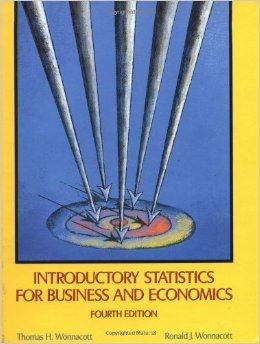
\includegraphics[scale=0.5]{./images/textbook.jpeg}
	\end{center}
	\centering
	Just get a used copy and save some money
\end{frame}

%%%%%%%%%%%%%%%%%%%%%%%%%%%%%%%%%%%%%%%%
\begin{frame}
\frametitle{Grading}
	\begin{enumerate}
		\item \alert{Default Scheme}
			\begin{align*}
			\text{Final Grade} &= (20\% \times \text{Quizzes}) + (20\% \times \text{Midterm 1})  
			\\
			&+ (20\% \times \text{Midterm 2}) + (40\% \times \text{Final})
			\end{align*}
		\item \alert{Participation Scheme (must opt-in)}
			\begin{align*}
			\text{Final Grade} &= (10\% \times \text{Participation}) + (10\% \times \text{Homework})
			\\
			&+ (10\% \times \text{Quizzes}) + (20\% \times \text{Midterm 1}) 
			\\
			&+ (20\% \times \text{Midterm 2}) + (30\% \times \text{Final})
			\end{align*}
	\end{enumerate}
\end{frame}

%%%%%%%%%%%%%%%%%%%%%%%%%%%%%%%%%%%%%%%%
\begin{frame}
\frametitle{Attendance}
	\begin{itemize}
		\item I will not take attendance, so show up if it's helpful
		\item If you opted into the ``Participation'' grading scheme, part of your score comes from 			how active you are in class, so ask questions and \alert{\textsc{participate}}!
	\end{itemize}
\end{frame}

%%%%%%%%%%%%%%%%%%%%%%%%%%%%%%%%%%%%%%%%
\begin{frame}
\frametitle{How Do I Do Well In the Course?}
	\begin{itemize}[<+- | alert@+>]
		\item Don't cram
		\item Learn concepts, don't memorize
		\item Review slides shortly after lecture
		\item Quizzes assess your fundamental understanding
		\item Do the homework
		\item Learn R\alert<7>{\only<7>{, seriously.}}
	\end{itemize}
\end{frame}

%%%%%%%%%%%%%%%%%%%%%%%%%%%%%%%%%%%%%%%%
\begin{frame}
\frametitle{Motivation}
	\begin{center}
		
\includegraphics[scale=0.6]{./images/uncle_sam.jpg}
	\end{center}
\end{frame}

%%%%%%%%%%%%%%%%%%%%%%%%%%%%%%%%%%%%%%%%
\begin{frame}
	\frametitle{Real Motivation}
	\href{run:./sound/Cave_Johnson_athletes.wav}{\beamergotobutton{Who's Ready to Make 			Some Science?}}
	\begin{center}
		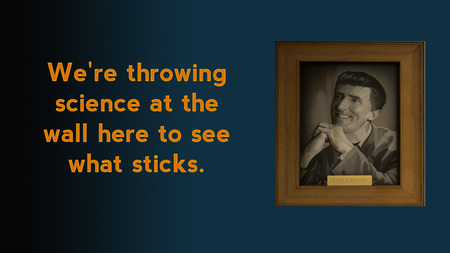
\includegraphics[scale=0.5]{./images/cave_johnson.jpg}
	\end{center}
\end{frame}

%%%%%%%%%%%%%%%%%%%%%%%%%%%%%%%%%%%%%%%%
\begin{frame}
	\frametitle{Real Life Examples}
	\begin{center}
		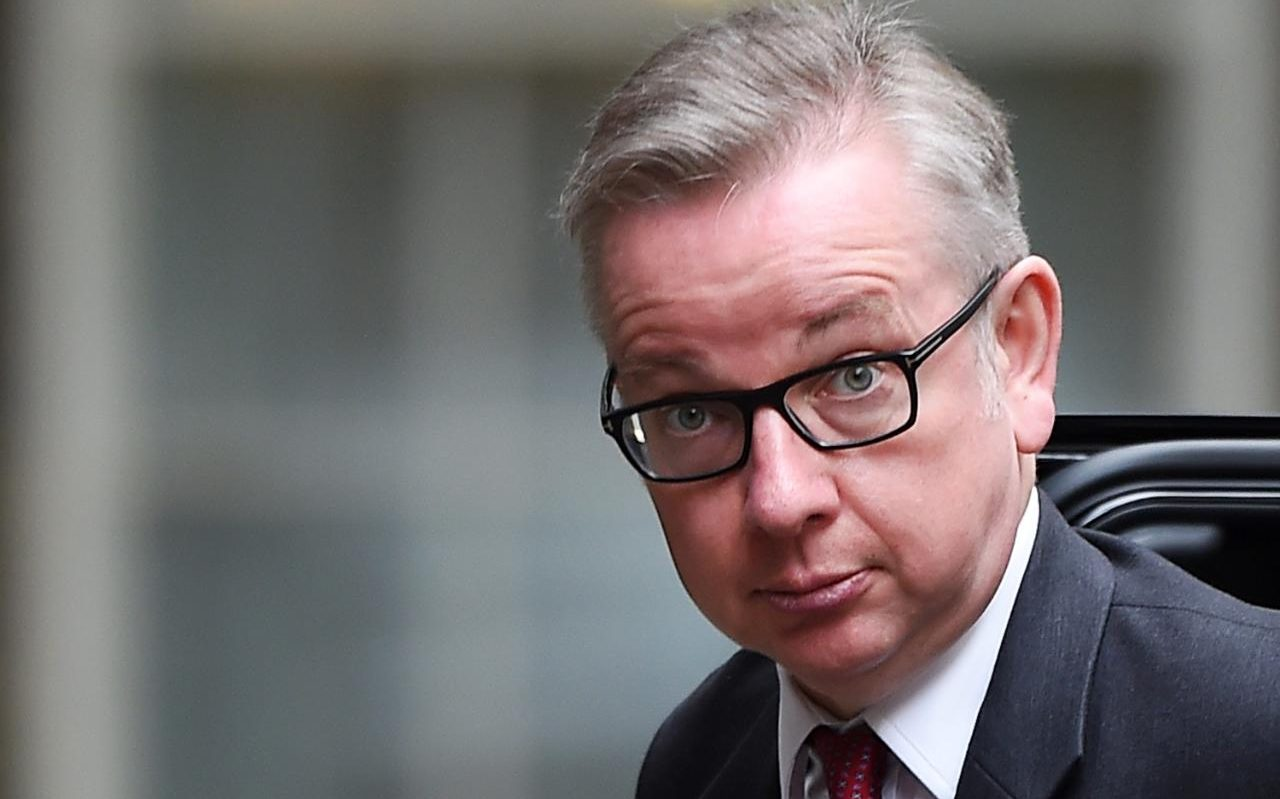
\includegraphics[scale=0.1]{./images/michael_gove.jpg}
	\end{center}
	\centering
	``People in this country have had enough of experts''
\end{frame}

%%%%%%%%%%%%%%%%%%%%%%%%%%%%%%%%%%%%%%%%
\begin{frame}
	\frametitle{Real Life Examples}
	\begin{center}
		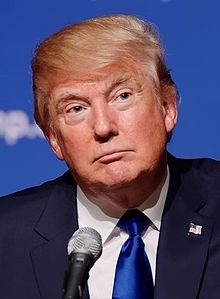
\includegraphics[scale=0.5]{./images/trump.jpg}
	\end{center}
	\centering
	``5.3 percent unemployment -- that is the biggest joke there is in this country. … The 				unemployment rate is probably 20 percent, but I will tell you, you have some great economists 		that will tell you it's a 30, 32. And the highest I've heard so far is 42 percent.''
\end{frame}

%%%%%%%%%%%%%%%%%%%%%%%%%%%%%%%%%%%%%%%%
\begin{frame}
\frametitle{Questions}
	\begin{itemize}[<+- | alert@+>]
		\item How many people are employed?
		\item How many people have a high school diploma/GED?
	\end{itemize}
\end{frame}

%%%%%%%%%%%%%%%%%%%%%%%%%%%%%%%%%%%%%%%%
\begin{frame}
\frametitle{Bad Statistics}
	\begin{itemize}
		\item Using this class as a representation of the U.S. population
		\begin{itemize}
			\item U.S. employment-population ratio is 59.7 percent
			\item 88 percent of adults (25 and older) have a high-school degree or equivalent
		\end{itemize}
	\end{itemize}
\end{frame}

%%%%%%%%%%%%%%%%%%%%%%%%%%%%%%%%%%%%%%%%
\begin{frame}
\frametitle{Good (Albeit Useless) Statistics}
	\begin{itemize}
		\item Using this class as a representation of this class
		\begin{itemize}
			\item X percent of Wednesday evening Econ 103 students are employed
			\item X percent of Wednesday evening Econ 103 students have a high school diploma 				or equivalent
		\end{itemize}
	\end{itemize}
\end{frame}

%%%%%%%%%%%%%%%%%%%%%%%%%%%%%%%%%%%%%%%%
\begin{frame}
\frametitle{Rule 1: Sample $\neq$ Population}
	\begin{center}
		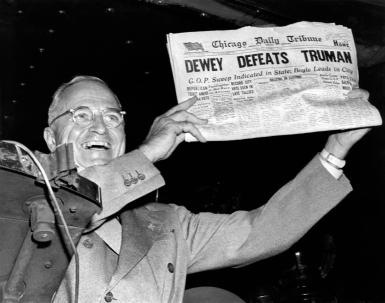
\includegraphics[scale=0.5]{./images/truman.jpg}
	\end{center}
	\centering
	How did this happen?
\end{frame}

%%%%%%%%%%%%%%%%%%%%%%%%%%%%%%%%%%%%%%%%
\begin{frame}
\frametitle{Definitions}
	\begin{itemize}
		\item \textbf{Population:} Complete set of all items of interest
		\item \textbf{Parameter:} A specific characteristic of a \textit{population}
		\item \textbf{Sample:} Observed subset of the \textit{population}
		\item \textbf{Statistic:} A specific characteristic of a \textit{sample}
		\item \textbf{Sample Size ($n$):} Number of items in the \textit{sample}
	\end{itemize} 
\end{frame}

%%%%%%%%%%%%%%%%%%%%%%%%%%%%%%%%%%%%%%%%
\begin{frame}
\frametitle{Essential Distinction You Must Remember!}
	\begin{figure}
		\centering
		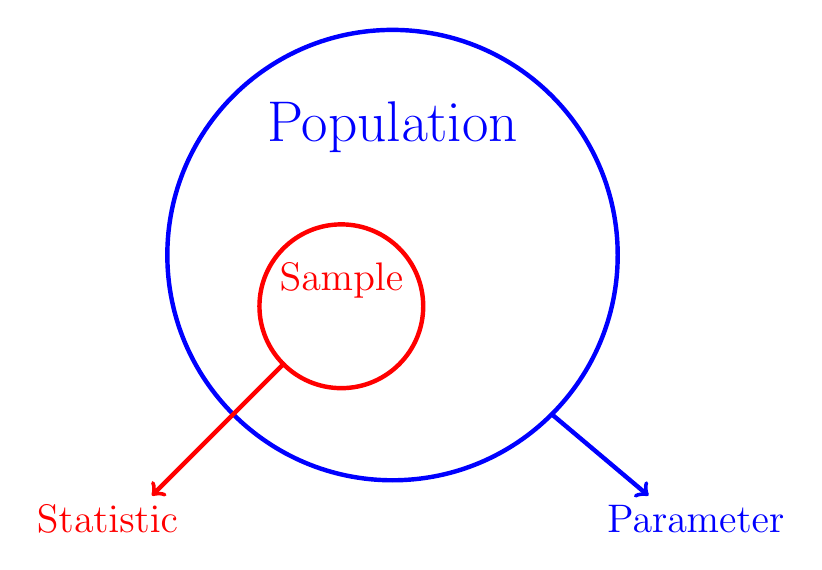
\begin{tikzpicture}[scale=1.3]
			\draw [blue, ultra thick] (0,0) circle [radius=2.2];
			\node [blue, font=\huge] at (0,1.25) {Population};
			\draw [blue, ultra thick, ->] (1.55,-1.55) -- (2.5,-2.35);
			\draw [red, ultra thick] (-0.5, -0.5) circle [radius=0.8];
			\node [blue, font =\Large, below right] at (2, -2.35) {Parameter};
			\node [red, font=\Large] at (-0.5, -0.25) {Sample};
			\draw [red, ultra thick, ->] (-1.05, -1.05) -- (-2.35, -2.35);
			\node [red, font =\Large, below left] at (-2, -2.35) {Statistic};
		\end{tikzpicture}
	\end{figure}
\end{frame}

%%%%%%%%%%%%%%%%%%%%%%%%%%%%%%%%%%%%%%%%
\begin{frame}
\frametitle{Kinds of Statistics}
	\begin{itemize}
		\item \textbf{Descriptive Statistics:} Graphical and numerical summaries of data
		\item \textbf{Inferential Statistics:} Using data to estimate, predict, and quantify 					uncertainty
	\end{itemize}
\end{frame}

%%%%%%%%%%%%%%%%%%%%%%%%%%%%%%%%%%%%%%%%
\begin{frame}
\frametitle{Course Outline}
	\begin{enumerate}
		\item Descriptive Statistics: summarize data
			\begin{itemize}
				\item Summary Statistics
				\item Graphics
			\end{itemize}
		\item Probability: Population $\rightarrow$ Sample
			\begin{itemize}
				\item Using information about the population to predict properties of a sample
				\item Deductive: ``safe'' argument
					\begin{itemize}
						\item All Smurfs are blue. Papa Smurf is a Smurf. Papa Smurf must be blue.
					\end{itemize}
			\end{itemize}
		\item Statistics: Sample $\rightarrow$ Population
			\begin{itemize}
				\item Using information about the sample to predict properties of the population
				\item Inductive: ``risky'' argument
					\begin{itemize}
						\item I've only seen blue Smurfs, so all Smurfs must be blue.
					\end{itemize}
			 \end{itemize}
	\end{enumerate}
\end{frame}

%%%%%%%%%%%%%%%%%%%%%%%%%%%%%%%%%%%%%%%%
\begin{frame}
\frametitle{Why Do Statistics?}
	\begin{itemize}[<+- | alert@+>]
		\item \textbf{Ockham's Razor:} If we can predict everything based on the population, just 			get data on the population and call it a day, right? How hard can this really be?
		\item What's wrong with this reasoning?
		\begin{itemize}[<+- | alert@+>]
			\item \textbf{Limited resources:} Surveying the whole population is expensive and 					usually infeasible
			\item \textbf{Scarcity:} Sometimes only a small sample is available
			\item \textbf{Destructive testing:} Rating car parts for durability requires testing them 				until they break. If you tested every part, you'd have no parts to use in cars.
			\item \textbf{Error reduction:} Getting data on the whole population could aggravate 				measurement error if done improperly
		\end{itemize}
	\end{itemize}	
\end{frame}

%%%%%%%%%%%%%%%%%%%%%%%%%%%%%%%%%%%%%%%%
\begin{frame}
\frametitle{Sampling and Nonsampling Error}
In statistics we use samples to learn about populations, but samples almost never are \emph{exactly} like the population they are drawn from.
	\begin{enumerate}
		\item Sampling Error 
			\begin{itemize}
				\item \emph{Random} differences between sample and population
				\item Cancel out on average
				\item Decreases as sample size grows
			\end{itemize}
		\item Nonsampling Error
			\begin{itemize}
				\item \emph{Systematic} differences between sample and population 
				\item Does \emph{not} cancel out on average
				\item Does \emph{not} decrease as sample size grows
			\end{itemize}
	\end{enumerate}
\end{frame}

%%%%%%%%%%%%%%%%%%%%%%%%%%%%%%%%%%%%%%%%
\begin{frame}
\frametitle{Illustrative Example}
	\begin{center}
		\includegraphics[scale = 0.25]{./images/LiteraryDigest}
	\end{center}
\end{frame}

%%%%%%%%%%%%%%%%%%%%%%%%%%%%%%%%%%%%%%%%
\begin{frame}
\frametitle{Literary Digest -- 1936 Presidential Election Poll}
	\begin{center}
		\includegraphics[scale = 0.3]{./images/FDR}
		\includegraphics[scale = 1.67]{./images/Landon}\\
		\small FDR versus Kansas Gov.\ Alf Landon
	\end{center}
	\normalsize

	\begin{block}{Data}
		Sent out over 10 million ballots to those on auto registries and phone books. 
		
		2.4 million replied (Compared to  less than $45$ million votes cast in actual election)
	\end{block}
	
	\begin{block}{Prediction}
		Landslide for Landon: \emph{Landonslide},  if you will.
	\end{block}
\end{frame}

%%%%%%%%%%%%%%%%%%%%%%%%%%%%%%%%%%%%%%%%
\begin{frame}
\frametitle{What Could Go Wrong?}
	\begin{center}
		\includegraphics[scale = 0.3]{./images/FDR}
		\includegraphics[scale = 1.67]{./images/Landon}\\
		\small FDR versus Kansas Gov.\ Alf Landon
	\end{center}
	\normalsize
	\begin{center}
		\begin{tabular}{lcc}
									&Roosevelt		&Landon\\
		Literary Digest Prediction: 	&41\% 			& \alert{57\%}\\
		\onslide<3>{	Actual Result: 				&\alert{61\%} 	& 37\%}
		\end{tabular}
	\end{center}
	
	\onslide<2>{The rest is history. President Landon joined the ranks of forgettable presidents like 		Millard Fillmore and William Henry Harrison}
	\onslide<3>{\alert{\textbf{Oops}\ldots}}
\end{frame}

%%%%%%%%%%%%%%%%%%%%%%%%%%%%%%%%%%%%%%%%
\begin{frame}
\frametitle{What Went Wrong? \emph{Non-sampling Error (aka Bias)}}
	\begin{block}{Biased Sample}
		Sampled car owners and those with telephones
	\end{block}
	
	\begin{block}{Non-response Bias}
	Even if sample is unbiased, can't force people to reply.
		\begin{itemize}
			\item Among those who recieved a ballot, Landon supporters were more likely to reply.
		\end{itemize}
	\end{block}
	\alert{In this case, neither effect \emph{alone} was enough to throw off the result but together 		they did.}
	
	\tiny{Source: \href{http://www.jstor.org/stable/10.2307/2749114}{\fbox{Squire (1988)}}}
\end{frame}

%%%%%%%%%%%%%%%%%%%%%%%%%%%%%%%%%%%%%%%%
\begin{frame}
\frametitle{How Do You Get an Unbiased Sample?}
	\begin{block}{Simple Random Sample}	
		Each member of population is chosen strictly by chance, so that: (1) selection of one 					individual doesn't influence selection of any other, (2) each individual is just as likely to be 			chosen, (3) every possible sample of size $n$ has the same chance of selection.	
	\end{block}
	
	\begin{block}{What about non-response bias?}
	\end{block}
\end{frame}

%%%%%%%%%%%%%%%%%%%%%%%%%%%%%%%%%%%%%%%%
\begin{frame}
\frametitle{``Americans Divided on Outlook for Next Generation''}
	\vspace{1em}
	\begin{quote}
		PRINCETON, NJ -- Americans are evenly divided about whether it is likely (49\%) or unlikely 			(50\%) that the next generation of youth in the country will have a better life than their 				parents. That is a slightly more positive assessment than in early 2011, when the slight 				majority, 55\%, thought it was unlikely the next generation would achieve this goal.
	\end{quote}
	\tiny{Source: \href{http://www.gallup.com/poll/159737/americans-divided-outlook-next-generation.aspx}{\fbox{Gallup}}}	
\end{frame}

%%%%%%%%%%%%%%%%%%%%%%%%%%%%%%%%%%%%%%%%
\begin{frame}
\frametitle{Example of Sampling Error}
	``...evenly divided about whether it is likely (49\%) or unlikely (50\%) that the next generation 		of youth in the country will have a better life...''
	\vspace{2em}
	\begin{quote}
		Results for this USA Today/Gallup poll are based on telephone interviews conducted Dec. 			14-17, 2012, with a \alert{random sample of 1025 adults}, aged 18 and older, living in all 50 			U.S. states and the District of Columbia. For results based on the total sample of national 			adults, one can say with \alert{95\% confidence that the maximum margin of sampling 				error is ±4 percentage points}.
	\end{quote}
\end{frame}

%%%%%%%%%%%%%%%%%%%%%%%%%%%%%%%%%%%%%%%%
\begin{frame}
\frametitle{Quantifying Sampling Error}
	$$Margin of Error (ME) \approx 2 \sqrt{P(1-P)/n}$$
	We report: $P \pm ME$
\end{frame}

%%%%%%%%%%%%%%%%%%%%%%%%%%%%%%%%%%%%%%%%
\begin{frame}
\frametitle{Swimming Pools and Lead Poisoning}
	Ask random sample of parents if they have an in-ground swimming pool and whether their   			child contracted lead poisoning. Compare those who had pools to those who did not.
	\vspace{1em}
	Would this procedure:
		\begin{enumerate}[(a)]
			\item Overstate health benefits of swimming (or really, having a swimming pool)
			\item Correctly identify health benefits of swimming
			\item Understate health benefits of swimming
		\end{enumerate}
\end{frame}

%%%%%%%%%%%%%%%%%%%%%%%%%%%%%%%%%%%%%%%%
\begin{frame}
\frametitle{Problem}
	Parents who own swimming pools may differ systematically from those who don't in 				\emph{other ways} that impact child's chance of getting lead poisoning!
	\vspace{2em}
	\begin{alertblock}{Wealth influences one's ability to have a swimming pool and to live in a house without lead paint.}
	\end{alertblock}
\end{frame}

%%%%%%%%%%%%%%%%%%%%%%%%%%%%%%%%%%%%%%%%
\begin{frame}
\frametitle{Confounder}
	Factor than influences both outcomes and whether subjects are treated or not. Masks true 			effect of treatment.
\end{frame}

%%%%%%%%%%%%%%%%%%%%%%%%%%%%%%%%%%%%%%%%
\begin{frame}
\frametitle{Properly Determining Treatment Effectiveness: Randomized Experiments}
	\begin{itemize}
		\item Start with group of experimental subjects
		\item Randomly assign one group to get the ``treatment'' and the other gets nothing (i.e. the ``control'' group)
		\item Random assignment neutralizes the chance of confounding factors since groups are 			initially equal, on average, and only difference is the treatment.
	\end{itemize}
	\alert{Double-blind randomized trials are the gold standard}
\end{frame}

%%%%%%%%%%%%%%%%%%%%%%%%%%%%%%%%%%%%%%%%
\begin{frame}
\frametitle{Double-Blind Randomized Trial}
\begin{figure}
\centering
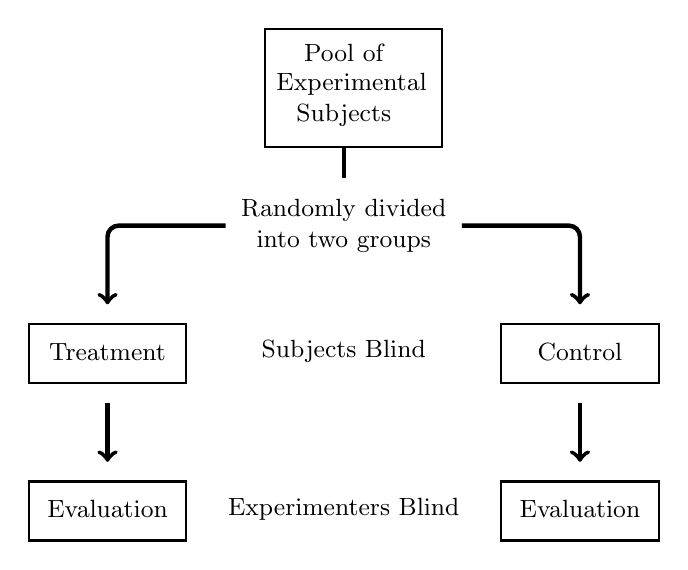
\begin{tikzpicture}
	\draw [thick] (0,0) rectangle (2.25,1.5);
	\draw [ultra thick] (1,0) -- (1,-0.4);
	\draw [ultra thick, ->, rounded corners] (2.5,-1) -- (4,-1) -- (4, -2);
	\draw [ultra thick, ->, rounded corners] (-0.5,-1) -- (-2,-1) -- (-2, -2);
	\draw [ultra thick, ->] (-2, -3.25) -- (-2, -4); 
	\draw [ultra thick, ->] (4, -3.25) -- (4, -4); 
	\draw [thick] (3,-2.25) rectangle (5,-3);
	\draw [thick] (3,-4.25) rectangle (5,-5);
	\draw [thick] (-3,-2.25) rectangle (-1,-3);
	\draw [thick] (-3,-4.25) rectangle (-1,-5);
	\node [font=\small] at (1,1.2) {Pool of};
	\node [font=\small] at (1.1,0.8) {Experimental};
	\node [font=\small] at (1,0.4) {Subjects};
	\node [font=\small] at (1,-0.8) {Randomly divided};
	\node [font=\small] at (1,-1.2) {into two groups};
	\node [font=\small] at (1,-2.6) {Subjects Blind};
	\node [font=\small] at (1,-4.6) {Experimenters Blind};
	\node [font=\small] at (4,-2.6) {Control};
	\node [font=\small] at (4,-4.6) {Evaluation};
	\node [font=\small] at (-2,-2.6) {Treatment};
	\node [font=\small] at (-2,-4.6) {Evaluation};
\end{tikzpicture}
\end{figure}
\end{frame}

%%%%%%%%%%%%%%%%%%%%%%%%%%%%%%%%%%%%%%%%
\begin{frame}
\frametitle{Gold Standard: Randomized, Double-blind Experiment}
	\begin{quote}
		Randomized blind experiments ensure that on average the two groups are initially equal, and continue to be treated equally. Thus a fair comparison is possible.
	\end{quote}
	
	\vspace{2em}
	\begin{alertblock}{Randomized, double-blind experiments are generally the best way to untangle causation.}
	\end{alertblock}
\end{frame}

%%%%%%%%%%%%%%%%%%%%%%%%%%%%%%%%%%%%%%%%
\begin{frame}
\frametitle{Randomized Trials and Real Life}
	\alert{Ockham's Razor II:} Randomize everything and fix this whole causation/correlation problem!
	\begin{block}{What Shall We Solve?}
		\begin{itemize}[<+->]
			\item Does gender affect one's wages?
			\item Does the defendant's race affect their sentencing?
			\item Does spanking cause criminality?
		\end{itemize}
	\end{block}
\end{frame}

%%%%%%%%%%%%%%%%%%%%%%%%%%%%%%%%%%%%%%%%
\begin{frame}
	\Huge{Randomization is not always possible, practical, or ethical.}
\end{frame}

%%%%%%%%%%%%%%%%%%%%%%%%%%%%%%%%%%%%%%%%
\begin{frame}
	\frametitle{Aperture Science and Randomized Trials}
	\begin{center}
		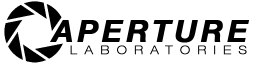
\includegraphics[scale=1]{./images/aperture.png}
	\end{center}
	\href{run:./sound/Cave_Johnson_mandatory_testing.wav}{\beamergotobutton{Mandatory Testing}}
	\href{run:./sound/Cave_Johnson_control1.wav}{\beamergotobutton{Control Groups}}
	\href{run:./sound/Cave_Johnson_control2.wav}{\beamergotobutton{Control Groups (ct'd)}}
\end{frame}

%%%%%%%%%%%%%%%%%%%%%%%%%%%%%%%%%%%%%%%%
\begin{frame}
\frametitle{How Can We Learn Anything Without Randomized Experiments?}
	\begin{block}{Observational Data}
		Data that do not come from a randomized experiment.	
	\end{block}
	\vspace{2em}
	\begin{alertblock}{It is very difficult to untangle cause and effect using observational data because of confounders.}
	\end{alertblock}
\end{frame}

%%%%%%%%%%%%%%%%%%%%%%%%%%%%%%%%%%%%%%%%
\begin{frame}
\frametitle{Does Racial Discrimination  Affect Criminal Sentencing?}
	\begin{quote}
	\footnotesize
		Social scientists have studied the issue for decades, but the seemingly simple question ``Does race affect sentencing?'' is surprisingly difficult to answer on the basis of empirical evidence.
		
		Abrams explains: \alert{``The most straightforward way you might look at it is to say, Let’s look at what sentences people get and see whether sentence length varies by race. If it looks like people of one race receive longer sentences than another, that might indicate that the criminal justice system is unfair. But the shortcoming to that approach is that it’s also possible that sentences can differ for many reasons; for example, it’s possible people of different races might have different criminal histories on average, and that could also explain the difference in sentence length.''}
	\end{quote}
	\tiny{Source: \href{https://www.law.upenn.edu/live/news/2170-new-study-by-professor-david-s-abrams-confirms}{\fbox{Penn Law Website}}}
\end{frame}

%%%%%%%%%%%%%%%%%%%%%%%%%%%%%%%%%%%%%%%%
\begin{frame}
\frametitle{Reducing Bias in Observational Studies}
	\begin{block}{Regression}
	Technique that allows us to remove influence of confounders. Works well if we can identify and gather data on all of them. But...
	\end{block}
\end{frame}

%%%%%%%%%%%%%%%%%%%%%%%%%%%%%%%%%%%%%%%%
\begin{frame}
\frametitle{Does Racial Discrimination  Affect Criminal Sentencing?}
	\footnotesize
	\begin{quote}
		To address that difficulty [confounders] social scientists have ... applied control variables to standard regression equations, a statistical method for identifying significant correlations between observed events. For instance, controlling for type of crime committed or for the defendant’s criminal history, researchers look to see whether the results of their equation still show racial disparity.\alert{``The problem with that is you still leave the possibility that any differences you see are due to unobserved variables, differences that might be there but that you can't control for''} Abrams says.``That might be demeanor in the courtroom, it might be the quality of the attorney you can afford, it might be some details about the crime that you might not capture in your data. If those things are correlated with race, which they probably are, you're not going to know whether the effect you think you're detecting is really race or is something else.''
	\end{quote}
	
	\tiny{Source: \href{https://www.law.upenn.edu/live/news/2170-new-study-by-professor-david-s-abrams-confirms}{\fbox{Penn Law Website}}}
\end{frame}

%%%%%%%%%%%%%%%%%%%%%%%%%%%%%%%%%%%%%%%%
\end{document}
